\pagestyle{empty}

% Capa
\begin{center}
\begin{tikzpicture}[remember picture,overlay]

    % Background with texture
    \node[inner sep=0] at (current page.center) {
        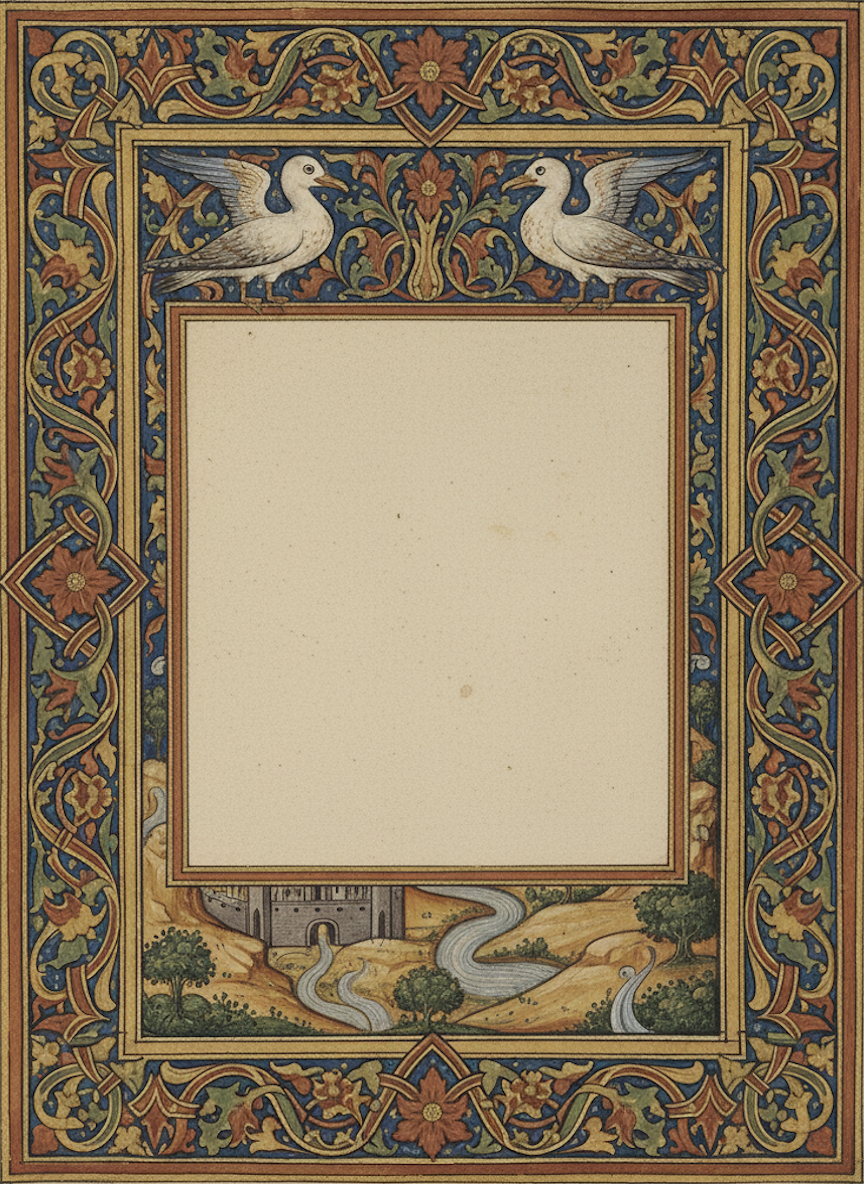
\includegraphics[
            width=1.02\paperwidth,
            height=1.02\paperheight
        ]{content/concept_art/title_page_2.png}
    };

    % Subtitle
    % \ifx\subtitle\undefined\else\if\relax\detokenize\expandafter{\subtitle}\relax\else
    % {\node[white, font=\Large, text width =\linewidth, align = center, anchor=north, below=8pt of title.south] {\textcolor{lightgray}{\scshape\large\subtitle}};}
    % \fi\fi

    % Center image
    % \node[anchor=center] at (current page.center) {
    %     
\includegraphics[width=0.6\paperwidth]{content/concept_art/acan_logo.png}
    % };

    % Publisher
    % \node[white, font=\Huge, anchor=south] (publisher) at ([yshift=32pt] current page.south) {\textcolor{white}{\scshape\large\publisher}};

    % Publisher logo
    \node[
        matrix,                   % This node will act as a container
        at=(current page.center), % Position the entire matrix at the page center
        yshift=3cm,               % Move Author and Title up together
        row sep=20pt,             % Default vertical space between rows (adjust as needed)
        xshift=0.0\paperwidth
    ]
    {
        % Row 1: Author
        \node[text width=\linewidth, align=center] {
            \textcolor{black}{\carolingian\scshape\large\authorname}
        }; \\ % End of the first row
        % Row 2: Title
        \node[text width=0.9\linewidth, align=center] (coverTitle) {
            \protect\contour{customgold}{\textcolor{ManuscriptRed}{\carolingian\scshape\Huge\booktitle}}
        }; \\ % End of the second row
    };

    % Subtitle (conditionally included)
    \ifdefined\subtitle
        \if\relax\detokenize\expandafter{\subtitle}\relax
        \else
            \node[text width=0.8\linewidth, align=center, below=12pt of coverTitle.south] {
                \protect\contour{customgold}{\textcolor{ManuscriptRed}{\carolingian\scshape\Large\subtitle}}
            };
        \fi
    \fi


    % Other information
    \ifx\translatorname\undefined
    \else
        \if\relax\detokenize\expandafter{\translatorname}\relax
        \else{
            \node[white, font=\Large, anchor=north, above=114pt of publisher.north] (translatedBy) {\textcolor{gray}{\itshape\large{Translated by}}};

            \node[white, font=\Large, anchor=south, below=2pt of translatedBy.south] (translatorAuthor) {\textcolor{lightgray}{\itshape\large\translatorname}};
            }
        \fi
    \fi
\end{tikzpicture}
\end{center}

\cleardoublepage

% Title page (back cover)
\begin{titlepage}
    \centering
    \newgeometry{top=1in,bottom=1in,right=0in,left=0in}
    \thispagestyle{empty}
    ~
    % Author
    \vspace{24pt}
    {\scshape\large \authorname\par}

    % Title
    \vspace{6pt}
    {\scshape\Huge \booktitle\par}

    % Subtitle
    \ifx\subtitle\undefined\else\if\relax\detokenize\expandafter{\subtitle}\relax\else
    {\vspace{6pt}
    {\scshape\large \subtitle\par}

    \vspace{\stretch{1.25}}}
    \fi\fi

    % Translator
    \ifx\translatorname\undefined\else\if\relax\detokenize\expandafter{\translatorname}\relax\else
    {{\itshape\large{Translated by}\par}
    \vspace{6pt}

    {\itshape\Large\translatorname\par}}
    \fi\fi

    % Publisher
    \vspace{\stretch{6}}
    {\Huge\scshape\large\publisher\par}
\end{titlepage}
